% Written by Claude Fable 5.2 (claude-fable-5-2) in the Claude app (cloud session), started by Andrei, 2026-11-14. Not human-reviewed.
% Status in the project's grades: computed + ai-proved. Not reviewed by another model. Not human-signed.
% Build: python3 gen_figs.py && latexmk -pdf path_proof.tex
\documentclass[11pt]{article}
\usepackage[margin=1in]{geometry}
\usepackage{amsmath,amssymb,amsthm}
\usepackage{enumitem}
\usepackage{tikz}
\usetikzlibrary{arrows.meta}
\usepackage[font=small,labelfont=bf]{caption}
\usepackage{booktabs}
\usepackage[hidelinks]{hyperref}

\newtheorem{theorem}{Theorem}
\newtheorem{lemma}[theorem]{Lemma}
\newtheorem{proposition}[theorem]{Proposition}
\newtheorem{corollary}[theorem]{Corollary}
\theoremstyle{definition}
\newtheorem{definition}[theorem]{Definition}
\newtheorem{example}[theorem]{Example}
\theoremstyle{remark}
\newtheorem{remark}[theorem]{Remark}

\newcommand{\E}{\textsf{E}}
\newcommand{\Ss}{\textsf{S}}
\newcommand{\W}{\mathcal{W}}

\definecolor{coralfill}{RGB}{250,226,216}\definecolor{coralline}{RGB}{216,90,48}
\definecolor{grayfill}{RGB}{241,239,232}\definecolor{grayline}{RGB}{136,135,128}
\definecolor{purpfill}{RGB}{206,203,246}\definecolor{purpline}{RGB}{83,74,183}
\definecolor{tealfill}{RGB}{159,225,203}\definecolor{tealline}{RGB}{15,110,86}
\tikzset{
  edge/.style={line width=0.5pt, black!70},
  act/.style={-{Stealth[length=2.2mm]}, line width=0.6pt},
  brace/.style={line width=0.5pt, black!55},
  ebox/.style={draw=coralline, fill=coralfill, line width=0.4pt, minimum width=0.42cm, minimum height=0.42cm, inner sep=0pt, font=\scriptsize},
  sbox/.style={draw=grayline, fill=grayfill, line width=0.4pt, minimum width=0.42cm, minimum height=0.42cm, inner sep=0pt, font=\scriptsize},
  eatom/.style={draw=coralline, line width=1.1pt, rounded corners=2.5pt},
  satom/.style={draw=black!60, line width=1.1pt, rounded corners=2.5pt},
  asymn/.style={circle, draw=purpline, fill=purpline!75, minimum size=7pt, inner sep=0pt},
  symn/.style={circle, draw=black!65, fill=white, line width=0.7pt, minimum size=7pt, inner sep=0pt},
  grid/.style={line width=0.3pt, black!18},
  diag/.style={line width=0.6pt, dashed, tealline},
  estep/.style={line width=1.7pt, coralline, line cap=round},
  sstep/.style={line width=1.7pt, black!62, line cap=round},
  fstep/.style={line width=1.7pt, tealline, line cap=round}
}

\title{Fuss--Catalan numbers modulo $p$\\ from rotations of path segments}
\author{Mighty Math Magicians $\cdot$ Caltech Mathathon 2026, Problem 137}
\date{14 November 2026}

\begin{document}
\maketitle
\vspace{-1.5em}

\begin{center}
\fbox{\parbox{0.92\textwidth}{\small\textbf{Provenance and status.} Written by Claude Fable 5.2 (Anthropic) in a chat session with
Andrei, on a question of his: can the theorem be proved by symmetries of lattice paths instead of trees?
In the project's grades the result below is \emph{computed} and \emph{ai-proved}. No other model has
reviewed the proof and no member of the team has signed it.}}
\end{center}

\section{Statement}

Let $p$ be a prime, $k\ge 1$, $q=p^k$, and $n\ge 1$. Put
\[
m=(q-1)n+1,\qquad N=n+m=qn+1,\qquad
C=C^{(q)}_n=\frac{1}{(q-1)n+1}\binom{qn}{n}=\frac1N\binom Nn .
\]
For an integer $u\ge 0$ write $u=\sum_i u_i p^i$ with digits $0\le u_i<p$, and $s_p(u)=\sum_i u_i$. Let
\[
t=\frac{s_p(m)-1}{p-1}.
\]

\begin{theorem}\label{thm:main}
$p^t$ divides $C$, and
\[
\frac{C}{p^t}\;\equiv\;\frac{(-1)^t}{\prod_j m_j!}\pmod p .
\]
In particular $C/p^t$ is not divisible by $p$.
\end{theorem}

The proof below uses lattice paths. Its steps run parallel to the steps of the tree proof (class sizes, a lower
bound from digit sums, minimal objects, a count modulo $p$), but the last step is a direct count: no cherry
collapse is needed. Section~\ref{sec:remarks} says what the argument does and does not give.

\section{Paths}

A \emph{path} is a sequence of unit steps $\E=(1,0)$ and $\Ss=(0,-1)$. We write a path as a word in the
letters $\E,\Ss$. Let $\W$ be the set of paths from $(0,m)$ to $(n,0)$: the words of length $N$ with $n$ letters
$\E$ and $m$ letters $\Ss$. So $|\W|=\binom Nn$.

\begin{lemma}[cyclic shifts]\label{lem:shift}
The $N$ cyclic shifts of a path in $\W$ are pairwise distinct. Hence the paths in $\W$, taken up to cyclic
shift, form $\binom Nn/N=C$ classes of $N$ paths each, and $|\W|=N\cdot C$.
\end{lemma}
\begin{proof}
If a shift by $r$ steps, $0<r<N$, fixes $w$, then $w$ consists of $N/g$ copies of a word of length $g=\gcd(r,N)<N$.
Then $N/g$ divides the number $n$ of letters $\E$, and it divides $N$. But $\gcd(n,N)=\gcd(n,qn+1)=1$, so
$N/g=1$, a contradiction.
\end{proof}

\begin{remark}[paths under the line]\label{rem:dyck}
$C$ also counts the paths from $(0,(q-1)n)$ to $(n,0)$ that stay weakly under the straight line through these two
points. By the cycle lemma, each class of Lemma~\ref{lem:shift} contains exactly one path of the form $\Ss v$ with $v$
such a path (Figure~\ref{fig:models}). We do not use this; we checked it by computer in small cases.
\end{remark}

\begin{figure}[ht]
\centering
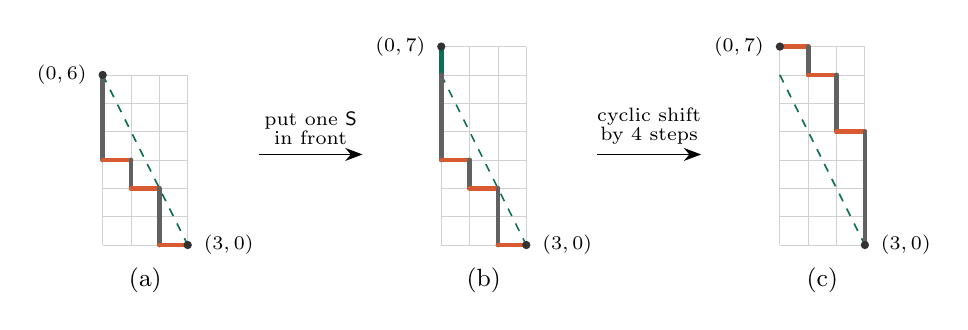
\begin{tikzpicture}
% Generated by gen_figs.py. Claude Fable 5.2 in the Claude app, started by Andrei, 2026-11-14. Not human-reviewed.
\draw[grid] (0.000,0.000) -- (0.000,2.160);
\draw[grid] (0.360,0.000) -- (0.360,2.160);
\draw[grid] (0.720,0.000) -- (0.720,2.160);
\draw[grid] (1.080,0.000) -- (1.080,2.160);
\draw[grid] (0.000,0.000) -- (1.080,0.000);
\draw[grid] (0.000,0.360) -- (1.080,0.360);
\draw[grid] (0.000,0.720) -- (1.080,0.720);
\draw[grid] (0.000,1.080) -- (1.080,1.080);
\draw[grid] (0.000,1.440) -- (1.080,1.440);
\draw[grid] (0.000,1.800) -- (1.080,1.800);
\draw[grid] (0.000,2.160) -- (1.080,2.160);
\draw[diag] (0.000,2.160) -- (1.080,0.000);
\draw[sstep] (0.000,2.160) -- (0.000,1.800);
\draw[sstep] (0.000,1.800) -- (0.000,1.440);
\draw[sstep] (0.000,1.440) -- (0.000,1.080);
\draw[estep] (0.000,1.080) -- (0.360,1.080);
\draw[sstep] (0.360,1.080) -- (0.360,0.720);
\draw[estep] (0.360,0.720) -- (0.720,0.720);
\draw[sstep] (0.720,0.720) -- (0.720,0.360);
\draw[sstep] (0.720,0.360) -- (0.720,0.000);
\draw[estep] (0.720,0.000) -- (1.080,0.000);
\fill[black!80] (0.000,2.160) circle (1.5pt);
\fill[black!80] (1.080,0.000) circle (1.5pt);
\node[font=\small] at (0.54,-0.45) {(a)};
\node[font=\scriptsize,anchor=east] at (-0.08,2.16) {$(0,6)$};
\node[font=\scriptsize,anchor=west] at (1.16,0) {$(3,0)$};
\draw[grid] (4.300,0.000) -- (4.300,2.520);
\draw[grid] (4.660,0.000) -- (4.660,2.520);
\draw[grid] (5.020,0.000) -- (5.020,2.520);
\draw[grid] (5.380,0.000) -- (5.380,2.520);
\draw[grid] (4.300,0.000) -- (5.380,0.000);
\draw[grid] (4.300,0.360) -- (5.380,0.360);
\draw[grid] (4.300,0.720) -- (5.380,0.720);
\draw[grid] (4.300,1.080) -- (5.380,1.080);
\draw[grid] (4.300,1.440) -- (5.380,1.440);
\draw[grid] (4.300,1.800) -- (5.380,1.800);
\draw[grid] (4.300,2.160) -- (5.380,2.160);
\draw[grid] (4.300,2.520) -- (5.380,2.520);
\draw[diag] (4.300,2.160) -- (5.380,0.000);
\draw[fstep] (4.300,2.520) -- (4.300,2.160);
\draw[sstep] (4.300,2.160) -- (4.300,1.800);
\draw[sstep] (4.300,1.800) -- (4.300,1.440);
\draw[sstep] (4.300,1.440) -- (4.300,1.080);
\draw[estep] (4.300,1.080) -- (4.660,1.080);
\draw[sstep] (4.660,1.080) -- (4.660,0.720);
\draw[estep] (4.660,0.720) -- (5.020,0.720);
\draw[sstep] (5.020,0.720) -- (5.020,0.360);
\draw[sstep] (5.020,0.360) -- (5.020,0.000);
\draw[estep] (5.020,0.000) -- (5.380,0.000);
\fill[black!80] (4.300,2.520) circle (1.5pt);
\fill[black!80] (5.380,0.000) circle (1.5pt);
\node[font=\small] at (4.84,-0.45) {(b)};
\node[font=\scriptsize,anchor=east] at (4.22,2.52) {$(0,7)$};
\node[font=\scriptsize,anchor=west] at (5.46,0) {$(3,0)$};
\draw[grid] (8.600,0.000) -- (8.600,2.520);
\draw[grid] (8.960,0.000) -- (8.960,2.520);
\draw[grid] (9.320,0.000) -- (9.320,2.520);
\draw[grid] (9.680,0.000) -- (9.680,2.520);
\draw[grid] (8.600,0.000) -- (9.680,0.000);
\draw[grid] (8.600,0.360) -- (9.680,0.360);
\draw[grid] (8.600,0.720) -- (9.680,0.720);
\draw[grid] (8.600,1.080) -- (9.680,1.080);
\draw[grid] (8.600,1.440) -- (9.680,1.440);
\draw[grid] (8.600,1.800) -- (9.680,1.800);
\draw[grid] (8.600,2.160) -- (9.680,2.160);
\draw[grid] (8.600,2.520) -- (9.680,2.520);
\draw[diag] (8.600,2.160) -- (9.680,0.000);
\draw[estep] (8.600,2.520) -- (8.960,2.520);
\draw[sstep] (8.960,2.520) -- (8.960,2.160);
\draw[estep] (8.960,2.160) -- (9.320,2.160);
\draw[sstep] (9.320,2.160) -- (9.320,1.800);
\draw[sstep] (9.320,1.800) -- (9.320,1.440);
\draw[estep] (9.320,1.440) -- (9.680,1.440);
\draw[sstep] (9.680,1.440) -- (9.680,1.080);
\draw[sstep] (9.680,1.080) -- (9.680,0.720);
\draw[sstep] (9.680,0.720) -- (9.680,0.360);
\draw[sstep] (9.680,0.360) -- (9.680,0.000);
\fill[black!80] (8.600,2.520) circle (1.5pt);
\fill[black!80] (9.680,0.000) circle (1.5pt);
\node[font=\small] at (9.14,-0.45) {(c)};
\node[font=\scriptsize,anchor=east] at (8.52,2.52) {$(0,7)$};
\node[font=\scriptsize,anchor=west] at (9.76,0) {$(3,0)$};
\draw[act] (1.98,1.15) -- node[above,font=\scriptsize,align=center]{put one \textsf{S}\\[-1pt] in front} (3.30,1.15);
\draw[act] (6.28,1.15) -- node[above,font=\scriptsize,align=center]{cyclic shift\\[-1pt] by $4$ steps} (7.60,1.15);

\end{tikzpicture}
\caption{$p=q=3$, $n=3$, so $m=7$, $N=10$, $C=12$. Steps $\E$ are drawn in coral, steps $\Ss$ in grey.
(a) A path from $(0,6)$ to $(3,0)$ under the dashed line. (b) The same path with one step $\Ss$ (teal) put in
front: a path in $\W$. (c) One of the other nine cyclic shifts of (b); none of them is of the form (b).}
\label{fig:models}
\end{figure}

\section{Segments, moves and classes}\label{sec:moves}

\emph{In Sections \ref{sec:moves}--\ref{sec:count}, $n,m\ge 0$ are arbitrary integers, $N=n+m$, and $\W$ is the set of words of length $N$
with $n$ letters $\E$ and $m$ letters $\Ss$. Only Section~\ref{sec:proof} uses $N=qn+1$.}

\paragraph{Segments.} Write $N=\sum_i N_ip^i$ in base $p$. Cut the positions $1,\dots,N$ into consecutive intervals:
$N_i$ intervals of length $p^i$ for each $i$, in order of decreasing length. These are the \emph{top segments}.
Cut every segment of length $p^h$, $h\ge1$, into $p$ consecutive \emph{sub-segments} of length $p^{h-1}$, and
repeat down to single steps. A \emph{segment} is a top segment or one of these iterated sub-segments.
The segments depend only on $N$ and $p$, not on the path. For a path $w$ and a segment $I$, the
\emph{piece} $w|_I$ is the part of $w$ on $I$.

When $N=qn+1$ the digits of $N$ are those of $n$, moved up by $k$ places, and a digit $1$ in place $0$:
\begin{equation}\label{eq:digitsN}
N_0=1,\qquad N_i=0\ \ (0<i<k),\qquad N_{k+i}=n_i .
\end{equation}
So there are $n_i$ top segments of length $q\,p^i$, followed by one single step.

\paragraph{Moves.} Let $I$ be a segment of length $p^h$, $h\ge 1$, and let $w|_I=u_1u_2\cdots u_p$, where $u_j$
is the piece on the $j$-th sub-segment. The \emph{move at $I$} replaces $u_1u_2\cdots u_p$ by $u_2\cdots u_pu_1$ and
changes nothing outside $I$. In words: cut this part of the path into $p$ equal pieces and glue them back in
rotated order (Figure~\ref{fig:moves}). A move permutes the steps, so it maps $\W$ to itself, and doing it $p$ times
gives back the path.

Two paths are \emph{equivalent} if a sequence of moves takes one to the other. All segments of length $p^h$ are
cut in the same way, so the same definition applies to words of length $p^h$: two such words $u,u'$ are
equivalent, $u\sim u'$, if, when they are placed on a segment $I$ of length $p^h$, moves at segments contained in $I$
take $u$ to $u'$. We write $[u]$ for the class of $u$, a set of words of length $p^h$. In particular we can
compare the pieces of a path on two different segments of the same length.

\begin{figure}[ht]
\centering
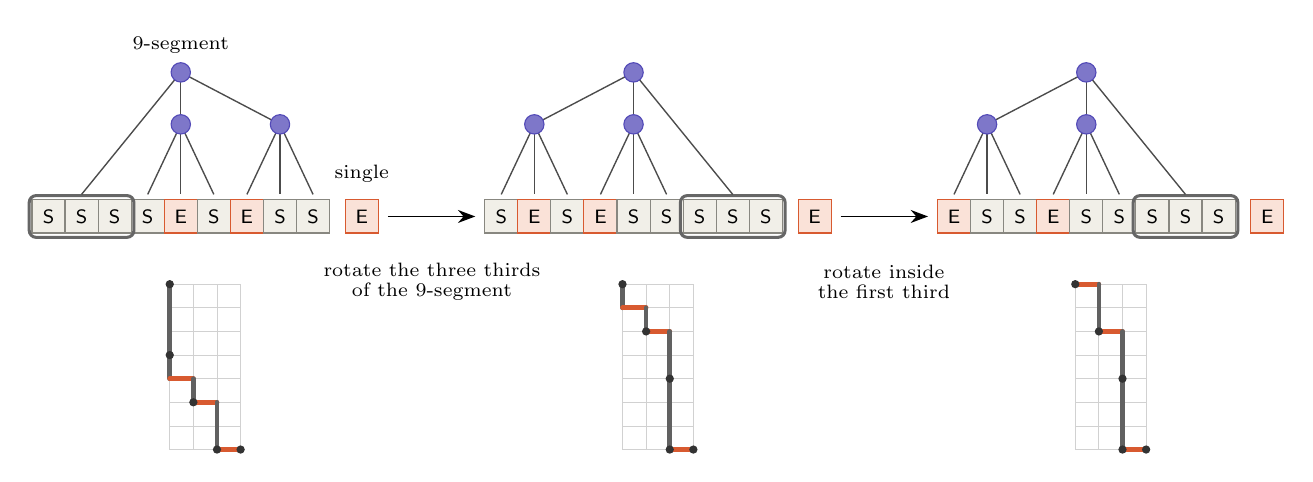
\begin{tikzpicture}
% Generated by gen_figs.py. Claude Fable 5.2 in the Claude app, started by Andrei, 2026-11-14. Not human-reviewed.
\node[sbox] at (0.210,0.210) {\textsf{S}};
\node[sbox] at (0.630,0.210) {\textsf{S}};
\node[sbox] at (1.050,0.210) {\textsf{S}};
\node[sbox] at (1.470,0.210) {\textsf{S}};
\node[ebox] at (1.890,0.210) {\textsf{E}};
\node[sbox] at (2.310,0.210) {\textsf{S}};
\node[ebox] at (2.730,0.210) {\textsf{E}};
\node[sbox] at (3.150,0.210) {\textsf{S}};
\node[sbox] at (3.570,0.210) {\textsf{S}};
\node[ebox] at (4.190,0.210) {\textsf{E}};
\draw[satom] (-0.035,-0.055) rectangle (1.295,0.475);
\draw[edge] (1.890,2.040) -- (0.630,0.490);
\draw[edge] (1.890,2.040) -- (1.890,1.380);
\draw[edge] (1.890,1.380) -- (1.470,0.490);
\draw[edge] (1.890,1.380) -- (1.890,0.490);
\draw[edge] (1.890,1.380) -- (2.310,0.490);
\node[asymn] at (1.890,1.380) {};
\draw[edge] (1.890,2.040) -- (3.150,1.380);
\draw[edge] (3.150,1.380) -- (2.730,0.490);
\draw[edge] (3.150,1.380) -- (3.150,0.490);
\draw[edge] (3.150,1.380) -- (3.570,0.490);
\node[asymn] at (3.150,1.380) {};
\node[asymn] at (1.890,2.040) {};
\draw[grid] (1.750,-2.750) -- (1.750,-0.650);
\draw[grid] (2.050,-2.750) -- (2.050,-0.650);
\draw[grid] (2.350,-2.750) -- (2.350,-0.650);
\draw[grid] (2.650,-2.750) -- (2.650,-0.650);
\draw[grid] (1.750,-2.750) -- (2.650,-2.750);
\draw[grid] (1.750,-2.450) -- (2.650,-2.450);
\draw[grid] (1.750,-2.150) -- (2.650,-2.150);
\draw[grid] (1.750,-1.850) -- (2.650,-1.850);
\draw[grid] (1.750,-1.550) -- (2.650,-1.550);
\draw[grid] (1.750,-1.250) -- (2.650,-1.250);
\draw[grid] (1.750,-0.950) -- (2.650,-0.950);
\draw[grid] (1.750,-0.650) -- (2.650,-0.650);
\draw[sstep] (1.750,-0.650) -- (1.750,-0.950);
\draw[sstep] (1.750,-0.950) -- (1.750,-1.250);
\draw[sstep] (1.750,-1.250) -- (1.750,-1.550);
\draw[sstep] (1.750,-1.550) -- (1.750,-1.850);
\draw[estep] (1.750,-1.850) -- (2.050,-1.850);
\draw[sstep] (2.050,-1.850) -- (2.050,-2.150);
\draw[estep] (2.050,-2.150) -- (2.350,-2.150);
\draw[sstep] (2.350,-2.150) -- (2.350,-2.450);
\draw[sstep] (2.350,-2.450) -- (2.350,-2.750);
\draw[estep] (2.350,-2.750) -- (2.650,-2.750);
\fill[black!80] (1.750,-1.550) circle (1.5pt);
\fill[black!80] (2.050,-2.150) circle (1.5pt);
\fill[black!80] (2.350,-2.750) circle (1.5pt);
\fill[black!80] (1.750,-0.650) circle (1.5pt);
\fill[black!80] (2.650,-2.750) circle (1.5pt);
\node[sbox] at (5.960,0.210) {\textsf{S}};
\node[ebox] at (6.380,0.210) {\textsf{E}};
\node[sbox] at (6.800,0.210) {\textsf{S}};
\node[ebox] at (7.220,0.210) {\textsf{E}};
\node[sbox] at (7.640,0.210) {\textsf{S}};
\node[sbox] at (8.060,0.210) {\textsf{S}};
\node[sbox] at (8.480,0.210) {\textsf{S}};
\node[sbox] at (8.900,0.210) {\textsf{S}};
\node[sbox] at (9.320,0.210) {\textsf{S}};
\node[ebox] at (9.940,0.210) {\textsf{E}};
\draw[edge] (7.640,2.040) -- (6.380,1.380);
\draw[edge] (6.380,1.380) -- (5.960,0.490);
\draw[edge] (6.380,1.380) -- (6.380,0.490);
\draw[edge] (6.380,1.380) -- (6.800,0.490);
\node[asymn] at (6.380,1.380) {};
\draw[edge] (7.640,2.040) -- (7.640,1.380);
\draw[edge] (7.640,1.380) -- (7.220,0.490);
\draw[edge] (7.640,1.380) -- (7.640,0.490);
\draw[edge] (7.640,1.380) -- (8.060,0.490);
\node[asymn] at (7.640,1.380) {};
\draw[satom] (8.235,-0.055) rectangle (9.565,0.475);
\draw[edge] (7.640,2.040) -- (8.900,0.490);
\node[asymn] at (7.640,2.040) {};
\draw[grid] (7.500,-2.750) -- (7.500,-0.650);
\draw[grid] (7.800,-2.750) -- (7.800,-0.650);
\draw[grid] (8.100,-2.750) -- (8.100,-0.650);
\draw[grid] (8.400,-2.750) -- (8.400,-0.650);
\draw[grid] (7.500,-2.750) -- (8.400,-2.750);
\draw[grid] (7.500,-2.450) -- (8.400,-2.450);
\draw[grid] (7.500,-2.150) -- (8.400,-2.150);
\draw[grid] (7.500,-1.850) -- (8.400,-1.850);
\draw[grid] (7.500,-1.550) -- (8.400,-1.550);
\draw[grid] (7.500,-1.250) -- (8.400,-1.250);
\draw[grid] (7.500,-0.950) -- (8.400,-0.950);
\draw[grid] (7.500,-0.650) -- (8.400,-0.650);
\draw[sstep] (7.500,-0.650) -- (7.500,-0.950);
\draw[estep] (7.500,-0.950) -- (7.800,-0.950);
\draw[sstep] (7.800,-0.950) -- (7.800,-1.250);
\draw[estep] (7.800,-1.250) -- (8.100,-1.250);
\draw[sstep] (8.100,-1.250) -- (8.100,-1.550);
\draw[sstep] (8.100,-1.550) -- (8.100,-1.850);
\draw[sstep] (8.100,-1.850) -- (8.100,-2.150);
\draw[sstep] (8.100,-2.150) -- (8.100,-2.450);
\draw[sstep] (8.100,-2.450) -- (8.100,-2.750);
\draw[estep] (8.100,-2.750) -- (8.400,-2.750);
\fill[black!80] (7.800,-1.250) circle (1.5pt);
\fill[black!80] (8.100,-1.850) circle (1.5pt);
\fill[black!80] (8.100,-2.750) circle (1.5pt);
\fill[black!80] (7.500,-0.650) circle (1.5pt);
\fill[black!80] (8.400,-2.750) circle (1.5pt);
\node[ebox] at (11.710,0.210) {\textsf{E}};
\node[sbox] at (12.130,0.210) {\textsf{S}};
\node[sbox] at (12.550,0.210) {\textsf{S}};
\node[ebox] at (12.970,0.210) {\textsf{E}};
\node[sbox] at (13.390,0.210) {\textsf{S}};
\node[sbox] at (13.810,0.210) {\textsf{S}};
\node[sbox] at (14.230,0.210) {\textsf{S}};
\node[sbox] at (14.650,0.210) {\textsf{S}};
\node[sbox] at (15.070,0.210) {\textsf{S}};
\node[ebox] at (15.690,0.210) {\textsf{E}};
\draw[edge] (13.390,2.040) -- (12.130,1.380);
\draw[edge] (12.130,1.380) -- (11.710,0.490);
\draw[edge] (12.130,1.380) -- (12.130,0.490);
\draw[edge] (12.130,1.380) -- (12.550,0.490);
\node[asymn] at (12.130,1.380) {};
\draw[edge] (13.390,2.040) -- (13.390,1.380);
\draw[edge] (13.390,1.380) -- (12.970,0.490);
\draw[edge] (13.390,1.380) -- (13.390,0.490);
\draw[edge] (13.390,1.380) -- (13.810,0.490);
\node[asymn] at (13.390,1.380) {};
\draw[satom] (13.985,-0.055) rectangle (15.315,0.475);
\draw[edge] (13.390,2.040) -- (14.650,0.490);
\node[asymn] at (13.390,2.040) {};
\draw[grid] (13.250,-2.750) -- (13.250,-0.650);
\draw[grid] (13.550,-2.750) -- (13.550,-0.650);
\draw[grid] (13.850,-2.750) -- (13.850,-0.650);
\draw[grid] (14.150,-2.750) -- (14.150,-0.650);
\draw[grid] (13.250,-2.750) -- (14.150,-2.750);
\draw[grid] (13.250,-2.450) -- (14.150,-2.450);
\draw[grid] (13.250,-2.150) -- (14.150,-2.150);
\draw[grid] (13.250,-1.850) -- (14.150,-1.850);
\draw[grid] (13.250,-1.550) -- (14.150,-1.550);
\draw[grid] (13.250,-1.250) -- (14.150,-1.250);
\draw[grid] (13.250,-0.950) -- (14.150,-0.950);
\draw[grid] (13.250,-0.650) -- (14.150,-0.650);
\draw[estep] (13.250,-0.650) -- (13.550,-0.650);
\draw[sstep] (13.550,-0.650) -- (13.550,-0.950);
\draw[sstep] (13.550,-0.950) -- (13.550,-1.250);
\draw[estep] (13.550,-1.250) -- (13.850,-1.250);
\draw[sstep] (13.850,-1.250) -- (13.850,-1.550);
\draw[sstep] (13.850,-1.550) -- (13.850,-1.850);
\draw[sstep] (13.850,-1.850) -- (13.850,-2.150);
\draw[sstep] (13.850,-2.150) -- (13.850,-2.450);
\draw[sstep] (13.850,-2.450) -- (13.850,-2.750);
\draw[estep] (13.850,-2.750) -- (14.150,-2.750);
\fill[black!80] (13.550,-1.250) circle (1.5pt);
\fill[black!80] (13.850,-1.850) circle (1.5pt);
\fill[black!80] (13.850,-2.750) circle (1.5pt);
\fill[black!80] (13.250,-0.650) circle (1.5pt);
\fill[black!80] (14.150,-2.750) circle (1.5pt);
\draw[act] (4.52,0.21) -- (5.63,0.21);
\node[font=\scriptsize,align=center] at (5.08,-0.62) {rotate the three thirds\\[-1pt] of the $9$-segment};
\draw[act] (10.27,0.21) -- (11.38,0.21);
\node[font=\scriptsize,align=center] at (10.82,-0.62) {rotate inside\\[-1pt] the first third};
\node[font=\scriptsize,anchor=south] at (1.89,2.16) {$9$-segment};
\node[font=\scriptsize,anchor=south] at (4.19,0.52) {single};

\end{tikzpicture}
\caption{$p=3$, $N=10$: one top segment of length $9$ and one single step. Top row: the path (b) of
Figure~\ref{fig:models} as a word, with its segments drawn as a tree, and two moves. A box drawn around several steps
is a monochromatic segment; purple discs are asymmetric segments (Definition~\ref{def:sym}). All three paths have
$d=3$. Bottom row: the same three paths in the plane; the dots cut the $9$-segment into thirds.}
\label{fig:moves}
\end{figure}

\begin{remark}
The moves generate a group of permutations of the $N$ positions: a product, over the top segments, of
iterated wreath products $\mathbb Z_p\wr\cdots\wr\mathbb Z_p$. It is the group of rotations of a forest of complete $p$-ary
trees whose leaves are the steps of the path. The classes are its orbits. By \cite[p.~239]{Kal} and
\cite[Section~2]{GL} (odd $p$ there), as recorded in the project's \texttt{references/README.md}, this group is a Sylow
$p$-subgroup of the symmetric group of the $N$ positions. We only need the classes.
\end{remark}

\begin{definition}\label{def:sym}
A piece is \emph{monochromatic} if all its steps are equal, and \emph{mixed} otherwise; we use the same words
for the segment carrying it. A segment $I$ of length $p^h$, $h\ge1$, is \emph{symmetric} for $w$ if the $p$
pieces of $w$ on its sub-segments are equivalent to one another, and \emph{asymmetric} otherwise. Single
steps count as symmetric. Monochromatic segments are symmetric. For a piece $u$ on a segment $I$, let $d(u)$ be the number of asymmetric segments contained in $I$, with $I$
itself; it depends only on the word $u$. For a path $w$, let $d(w)=\sum_Td(w|_T)$, the sum over the top segments
$T$: the number of all asymmetric segments.
\end{definition}

\begin{lemma}\label{lem:classes}
Let $I$ be a segment of length $p^h$, $h\ge 1$, and $u=u_1\cdots u_p$, $u'=u'_1\cdots u'_p$ two pieces on $I$.
Then $u\sim u'$ if and only if there is an $r$ with $u'_j\sim u_{j+r}$ for all $j$ (indices modulo $p$).
\end{lemma}
\begin{proof}
A move at a segment inside $I$ is either the move at $I$, which rotates the sequence of classes
$([u_1],\dots,[u_p])$, or a move inside one sub-segment, which does not change this sequence. So the
sequence of classes is determined by the class of $u$ up to rotation. Conversely, if $u'_j\sim u_{j+r}$ for all
$j$, apply the move at $I$ $r$ times and then moves inside the sub-segments.
\end{proof}

\begin{lemma}[class sizes]\label{lem:size}
The class of a piece $u$ has exactly $p^{\,d(u)}$ elements. The class of a path $w$ has
exactly $p^{\,d(w)}$ elements. In particular $d$ is constant on classes.
\end{lemma}
\begin{proof}
Let $u=u_1\cdots u_p$ be on a segment $I$ of length $p^h$. Induction on $h$; for $h=0$ both sides are $1$. Let $h\ge 1$. By Lemma~\ref{lem:classes},
$[u]$ is the union, over $r=0,\dots,p-1$, of the sets of words $v_1\cdots v_p$ with $v_j\in[u_{j+r}]$.
If $I$ is symmetric these $p$ sets coincide, so $|[u]|=\prod_j|[u_j]|$. If $I$ is asymmetric, the $p$ rotations
of the sequence $([u_1],\dots,[u_p])$ are pairwise distinct, because $p$ is prime and the sequence is not constant;
so the $p$ sets are disjoint and $|[u]|=p\prod_j|[u_j]|$. By induction $|[u_j]|=p^{d(u_j)}$, and
$d(u)=\sum_j d(u_j)$, plus $1$ if $I$ is asymmetric.
Finally, every move acts inside one top segment, so the class of $w$ is the product of the classes of its top pieces.
\end{proof}

\begin{figure}[ht]
\centering
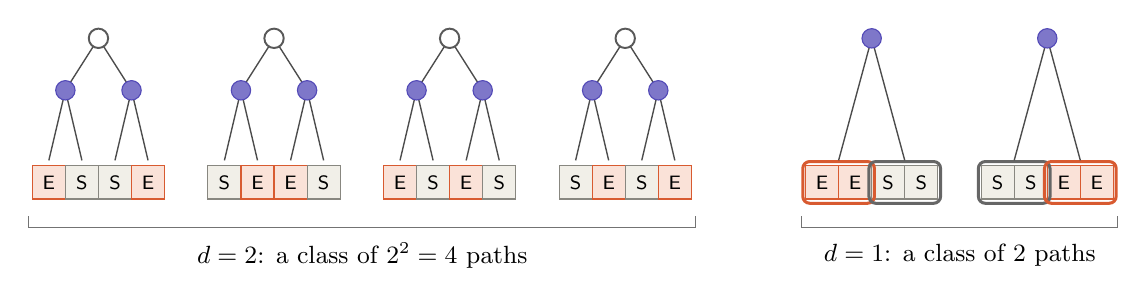
\begin{tikzpicture}
% Generated by gen_figs.py. Claude Fable 5.2 in the Claude app, started by Andrei, 2026-11-14. Not human-reviewed.
\node[ebox] at (0.210,0.210) {\textsf{E}};
\node[sbox] at (0.630,0.210) {\textsf{S}};
\node[sbox] at (1.050,0.210) {\textsf{S}};
\node[ebox] at (1.470,0.210) {\textsf{E}};
\draw[edge] (0.840,2.040) -- (0.420,1.380);
\draw[edge] (0.420,1.380) -- (0.210,0.490);
\draw[edge] (0.420,1.380) -- (0.630,0.490);
\node[asymn] at (0.420,1.380) {};
\draw[edge] (0.840,2.040) -- (1.260,1.380);
\draw[edge] (1.260,1.380) -- (1.050,0.490);
\draw[edge] (1.260,1.380) -- (1.470,0.490);
\node[asymn] at (1.260,1.380) {};
\node[symn] at (0.840,2.040) {};
\node[sbox] at (2.440,0.210) {\textsf{S}};
\node[ebox] at (2.860,0.210) {\textsf{E}};
\node[ebox] at (3.280,0.210) {\textsf{E}};
\node[sbox] at (3.700,0.210) {\textsf{S}};
\draw[edge] (3.070,2.040) -- (2.650,1.380);
\draw[edge] (2.650,1.380) -- (2.440,0.490);
\draw[edge] (2.650,1.380) -- (2.860,0.490);
\node[asymn] at (2.650,1.380) {};
\draw[edge] (3.070,2.040) -- (3.490,1.380);
\draw[edge] (3.490,1.380) -- (3.280,0.490);
\draw[edge] (3.490,1.380) -- (3.700,0.490);
\node[asymn] at (3.490,1.380) {};
\node[symn] at (3.070,2.040) {};
\node[ebox] at (4.670,0.210) {\textsf{E}};
\node[sbox] at (5.090,0.210) {\textsf{S}};
\node[ebox] at (5.510,0.210) {\textsf{E}};
\node[sbox] at (5.930,0.210) {\textsf{S}};
\draw[edge] (5.300,2.040) -- (4.880,1.380);
\draw[edge] (4.880,1.380) -- (4.670,0.490);
\draw[edge] (4.880,1.380) -- (5.090,0.490);
\node[asymn] at (4.880,1.380) {};
\draw[edge] (5.300,2.040) -- (5.720,1.380);
\draw[edge] (5.720,1.380) -- (5.510,0.490);
\draw[edge] (5.720,1.380) -- (5.930,0.490);
\node[asymn] at (5.720,1.380) {};
\node[symn] at (5.300,2.040) {};
\node[sbox] at (6.900,0.210) {\textsf{S}};
\node[ebox] at (7.320,0.210) {\textsf{E}};
\node[sbox] at (7.740,0.210) {\textsf{S}};
\node[ebox] at (8.160,0.210) {\textsf{E}};
\draw[edge] (7.530,2.040) -- (7.110,1.380);
\draw[edge] (7.110,1.380) -- (6.900,0.490);
\draw[edge] (7.110,1.380) -- (7.320,0.490);
\node[asymn] at (7.110,1.380) {};
\draw[edge] (7.530,2.040) -- (7.950,1.380);
\draw[edge] (7.950,1.380) -- (7.740,0.490);
\draw[edge] (7.950,1.380) -- (8.160,0.490);
\node[asymn] at (7.950,1.380) {};
\node[symn] at (7.530,2.040) {};
\draw[brace] (-0.05,-0.22) -- (-0.05,-0.36) -- (8.42,-0.36) -- (8.42,-0.22);
\node[font=\small] at (4.19,-0.72) {$d=2$: a class of $2^2=4$ paths};
\node[ebox] at (10.030,0.210) {\textsf{E}};
\node[ebox] at (10.450,0.210) {\textsf{E}};
\node[sbox] at (10.870,0.210) {\textsf{S}};
\node[sbox] at (11.290,0.210) {\textsf{S}};
\draw[eatom] (9.785,-0.055) rectangle (10.695,0.475);
\draw[edge] (10.660,2.040) -- (10.240,0.490);
\draw[satom] (10.625,-0.055) rectangle (11.535,0.475);
\draw[edge] (10.660,2.040) -- (11.080,0.490);
\node[asymn] at (10.660,2.040) {};
\node[sbox] at (12.260,0.210) {\textsf{S}};
\node[sbox] at (12.680,0.210) {\textsf{S}};
\node[ebox] at (13.100,0.210) {\textsf{E}};
\node[ebox] at (13.520,0.210) {\textsf{E}};
\draw[satom] (12.015,-0.055) rectangle (12.925,0.475);
\draw[edge] (12.890,2.040) -- (12.470,0.490);
\draw[eatom] (12.855,-0.055) rectangle (13.765,0.475);
\draw[edge] (12.890,2.040) -- (13.310,0.490);
\node[asymn] at (12.890,2.040) {};
\draw[brace] (9.77,-0.22) -- (9.77,-0.36) -- (13.78,-0.36) -- (13.78,-0.22);
\node[font=\small] at (11.78,-0.72) {$d=1$: a class of $2$ paths};

\end{tikzpicture}
\caption{$p=2$, one segment of length $4$, all $\binom42=6$ paths with two steps $\E$ and two steps $\Ss$.
Purple discs: asymmetric segments. White circles: symmetric mixed segments. In the class on the left the two halves
differ, but each half is a rotation of the other, so the whole segment is symmetric.
Here $6=2+4$: the lower bound of Section~\ref{sec:bound} is $d\ge1$, and there is one minimal class.}
\label{fig:classes}
\end{figure}

\begin{corollary}\label{cor:sum}
$\displaystyle\binom Nn=|\W|=\sum_{\text{classes}}p^{\,d}$, where $d$ is the common value of $d(w)$ on the class.
\end{corollary}

\section{A lower bound from digit sums}\label{sec:bound}

\begin{lemma}[carries]\label{lem:carries}
Define $c_0=0$ and $c_{i+1}=(n_i+m_i+c_i-N_i)/p$ for $i\ge 0$. Then every $c_i$ is $0$ or $1$, and
\[
c:=\sum_i c_i=\frac{s_p(n)+s_p(m)-s_p(N)}{p-1}.
\]
\end{lemma}
\begin{proof}
For an integer $u$ let $u^{(i)}$ be its remainder modulo $p^i$. Put $c'_i=(n^{(i)}+m^{(i)}-N^{(i)})/p^i$. This is an
integer, since $n+m=N$; it is $0$ or $1$, since $0\le n^{(i)}+m^{(i)}\le 2p^i-2$ and $0\le N^{(i)}\le p^i-1$.
Subtracting the definitions for $i$ and $i+1$ gives $n_i+m_i+c'_i=N_i+p\,c'_{i+1}$, and $c'_0=0$. So $c'_i=c_i$ for
all $i$. Summing $n_i+m_i+c_i=N_i+p\,c_{i+1}$ over $i$
(all $c_i$ with $p^i>N$ vanish) gives $s_p(n)+s_p(m)+c=s_p(N)+p\,c$.
\end{proof}

The number $c_i$ is the carry into digit $i$ when $n$ and $m$ are added in base $p$, and $c$ is the number of
carries. We say that integers $u^1,\dots,u^r\ge0$ \emph{add without carries} if in every digit place $i$ the sum of
their digits $\sum_j (u^j)_i$ is at most $p-1$; this sum is then the $i$-th digit of $u^1+\dots+u^r$.

\begin{lemma}[digit sums]\label{lem:digits}
\textup{(a)} $s_p(pu)=s_p(u)$. \textup{(b)} $s_p(u^1+\dots+u^r)\le s_p(u^1)+\dots+s_p(u^r)$, with equality
exactly when $u^1,\dots,u^r$ add without carries.
\end{lemma}
\begin{proof}
(a) is clear. For $r=2$, (b) is Lemma~\ref{lem:carries}: the difference of the two sides is $(p-1)c\ge0$, and $c=0$
exactly when $n_i+m_i\le p-1$ for all $i$. The general case follows by induction on $r$, adding one summand at a time.
\end{proof}

For a piece $u$ on a segment of length $p^h$ let $a(u)$ and $b(u)$ be its numbers of steps $\E$ and $\Ss$, so
$a(u)+b(u)=p^h$, and put
\[
\tau(u)=\frac{s_p(a(u))+s_p(b(u))-1}{p-1}.
\]

\begin{lemma}[lower bound for a piece]\label{lem:bound}
Let $u$ be a piece on a segment $I$, with sub-pieces $u_1,\dots,u_p$ if $I$ is longer than one step. Then
$d(u)\ge\tau(u)$. Equality holds exactly when either
$u$ is monochromatic, or the following three conditions hold: $I$ is asymmetric; equality holds for every
$u_j$; and $a(u_1),\dots,a(u_p)$ add without carries, and so do $b(u_1),\dots,b(u_p)$.
\end{lemma}
\begin{proof}
Induction on the length of $I$. Three cases.

\emph{$u$ monochromatic.} Then $d(u)=0$, and $\tau(u)=(0+s_p(p^h)-1)/(p-1)=0$.

\emph{$u$ mixed, $I$ symmetric.} The $u_j$ are equivalent to one another, so they have the same $a$, $b$ and $d$
(Lemma~\ref{lem:size}): $a(u)=p\,a(u_1)$, $b(u)=p\,b(u_1)$ and $d(u)=p\,d(u_1)$. As $u_1$ is mixed,
$\tau(u_1)>0$. So
\[
d(u)=p\,d(u_1)\ \ge\ p\,\tau(u_1)\ >\ \tau(u_1)=\tau(u),
\]
the last equality by Lemma~\ref{lem:digits}(a). Equality never holds in this case.

\emph{$I$ asymmetric.} Then, by induction and Lemma~\ref{lem:digits}(b),
\begin{align*}
d(u)=1+\sum_j d(u_j)\ &\ge\ 1+\sum_j\tau(u_j)
=1+\frac{\sum_j s_p(a(u_j))+\sum_j s_p(b(u_j))-p}{p-1}\\
&\ge\ 1+\frac{s_p(a(u))+s_p(b(u))-p}{p-1}=\tau(u),
\end{align*}
with equality exactly under the stated conditions.
\end{proof}

\begin{proposition}[lower bound]\label{prop:bound}
For every path $w\in\W$, $d(w)\ge c$, the number of carries. Equality holds exactly when equality holds in
Lemma~\ref{lem:bound} for every top piece, the numbers $a(w|_T)$ over the top segments $T$ add without carries,
and so do the numbers $b(w|_T)$.
\end{proposition}
\begin{proof}
There are $\sum_iN_i=s_p(N)$ top segments, $\sum_Ta(w|_T)=n$ and $\sum_Tb(w|_T)=m$. So by
Lemmas \ref{lem:bound} and \ref{lem:digits}(b),
\begin{align*}
d(w)=\sum_T d(w|_T)\ &\ge\ \sum_T\tau(w|_T)=\frac{\sum_Ts_p(a(w|_T))+\sum_Ts_p(b(w|_T))-s_p(N)}{p-1}\\
&\ge\ \frac{s_p(n)+s_p(m)-s_p(N)}{p-1}=c. \qedhere
\end{align*}
\end{proof}

We call $w$ \emph{minimal} if $d(w)=c$. By Lemma~\ref{lem:size} a class consists of minimal paths or contains
none. Corollary~\ref{cor:sum} and Proposition~\ref{prop:bound} give
\begin{equation}\label{eq:modp}
\binom Nn\;=\;p^{\,c}\,M+p^{\,c+1}R,\qquad M=\text{the number of classes of minimal paths},
\end{equation}
for some integer $R\ge0$. In particular $p^c$ divides $\binom Nn$.

\section{Minimal paths: atoms and carries}\label{sec:minimal}

\begin{definition}
An \emph{atom} of $w$ is a monochromatic segment that is a top segment or a sub-segment of a mixed segment. It is an
$\E$-atom or an $\Ss$-atom according to its steps. Every step of $w$ lies in exactly one atom: the largest
monochromatic segment containing it.
\end{definition}

\begin{lemma}[atoms are digits]\label{lem:atoms}
Let $w$ be minimal. Then every mixed segment is asymmetric, and for every $i$ the path $w$ has exactly $n_i$
$\E$-atoms and exactly $m_i$ $\Ss$-atoms of length $p^i$.
\end{lemma}
\begin{proof}
The first statement is part of the equality conditions of Lemma~\ref{lem:bound}, applied down the tree of segments. For the second, we show by induction
that for a piece $u$ with equality in Lemma~\ref{lem:bound}, the number of $\E$-atoms of length $p^i$ inside it is the
$i$-th digit of $a(u)$. If $u$ is monochromatic this is clear. If not, the atoms of $u$ are the atoms of
$u_1,\dots,u_p$, and the digits of $a(u_1),\dots,a(u_p)$ add up to the digits of $a(u)$ because these numbers
add without carries. The same argument at the top level (Proposition~\ref{prop:bound}) gives the digits of $n$, and the
same for $\Ss$ and $m$.
\end{proof}

\begin{lemma}[mixed segments are carries]\label{lem:mixed}
Let $w$ be minimal. For every $i$, the number of mixed segments of length $p^i$ is $c_i$. So $w$ has at most
one mixed segment of each length, and a mixed segment of length $p^i$ exactly when the addition $n+m=N$ carries
into digit $i$.
\end{lemma}
\begin{proof}
Let $x_i$ be the number of mixed segments of length $p^i$; $x_0=0$. Let $\mathcal R_i$ be the set of segments of
length $p^i$ that are top segments or sub-segments of a mixed segment. Then $|\mathcal R_i|=N_i+p\,x_{i+1}$. A member
of $\mathcal R_i$ is monochromatic, and then an atom, or mixed; and every atom and every mixed segment of length
$p^i$ lies in $\mathcal R_i$. By Lemma~\ref{lem:atoms},
\[
N_i+p\,x_{i+1}=n_i+m_i+x_i\qquad(i\ge0),\qquad x_0=0 .
\]
This is the recursion of Lemma~\ref{lem:carries}, so $x_i=c_i$ for all $i$.
\end{proof}

\section{Counting the minimal classes}\label{sec:count}

\begin{proposition}[count]\label{prop:count}
The number of minimal paths is $\prod_i\dfrac{(N_i+p\,c_{i+1})!}{n_i!\,m_i!}$. They form $M$ classes of $p^c$
paths each, where
\begin{equation}\label{eq:M}
M\cdot\prod_i n_i!\,m_i!\;=\;\prod_i\frac{(N_i+p\,c_{i+1})!}{p^{\,c_{i+1}}}\;\equiv\;(-1)^c\prod_iN_i!\pmod p .
\end{equation}
\end{proposition}
\begin{proof}
Build a minimal path from the longest segments down. By Lemma~\ref{lem:mixed} and its proof, at level $i$ there are
$N_i+p\,c_{i+1}$ \emph{slots}: the $N_i$ top segments of length $p^i$ and, if $c_{i+1}=1$, the $p$ sub-segments of
the unique mixed segment of length $p^{i+1}$, which was chosen at level $i+1$. Among the slots we choose $n_i$
to be $\E$-atoms, $m_i$ to be $\Ss$-atoms, and, if $c_i=1$, the remaining one to be mixed. The number of slots is
$n_i+m_i+c_i$, so this can be done in $(N_i+p\,c_{i+1})!/(n_i!\,m_i!)$ ways, whatever was chosen before.
At level $0$ there is nothing mixed, so the choices determine a word; it has $\sum_in_ip^i=n$ letters $\E$.

Every minimal path arises from exactly one sequence of choices (Lemmas \ref{lem:atoms} and \ref{lem:mixed}).
Conversely, let $w$ be built from any sequence of choices. The $p$ sub-segments of a segment chosen to be mixed
are slots of the next level; at most $n_{i-1}\le p-1$ of them are $\E$-atoms, at most $m_{i-1}\le p-1$ are
$\Ss$-atoms, and at most one is mixed. So its $p$ pieces are not all $\E$-atoms and not all $\Ss$-atoms. Going up from level $1$, this shows that a
segment chosen to be mixed really contains both letters. It is asymmetric: $p$ equivalent pieces
would be all monochromatic with the same letter, or all mixed, and both are excluded. All other segments are
monochromatic. Hence
$d(w)=\sum_ic_i=c$ and $w$ is minimal.

This proves the count of minimal paths. Each class of minimal paths has $p^c=\prod_ip^{c_{i+1}}$ elements
(Lemma~\ref{lem:size}), which gives the equality in \eqref{eq:M}. For the congruence: if $c_{i+1}=0$ the $i$-th
factor is $N_i!$. If $c_{i+1}=1$ it is
\[
\frac{(N_i+p)!}{p}=(p-1)!\,\prod_{j=1}^{N_i}(p+j)\;\equiv\;(p-1)!\,N_i!\;\equiv\;-N_i!\pmod p
\]
by Wilson's theorem.
\end{proof}

Together with \eqref{eq:modp} this gives the result for all binomial coefficients:

\begin{theorem}\label{thm:binom}
Let $n,m\ge0$, $N=n+m$, and let $c$ be the number of carries when $n$ and $m$ are added in base $p$. Then
$p^c$ divides $\binom Nn$ and
\[
\frac1{p^c}\binom Nn\;\equiv\;(-1)^c\prod_i\frac{N_i!}{n_i!\,m_i!}\pmod p .
\]
The right-hand side is not $0$ modulo $p$, so $p^c$ is the exact power of $p$ dividing $\binom Nn$.
\end{theorem}

\section{Proof of Theorem \ref{thm:main}}\label{sec:proof}

Let $N=qn+1$ and $m=(q-1)n+1$. By \eqref{eq:digitsN}, $s_p(N)=s_p(n)+1$ and $\prod_iN_i!=\prod_in_i!$. So the
number of carries is
\[
c=\frac{s_p(n)+s_p(m)-s_p(N)}{p-1}=\frac{s_p(m)-1}{p-1}=t ,
\]
and Theorem~\ref{thm:binom} gives $\binom Nn=p^tM+p^{t+1}R$ with $M\prod_jm_j!\equiv(-1)^t\pmod p$. By
Lemma~\ref{lem:shift}, $\binom Nn=N\cdot C$. As $p$ does not divide $N$, $p^t$ divides $C$. And as $N\equiv1\pmod p$,
\[
\frac C{p^t}\;\equiv\;\frac{N\cdot C}{p^t}\;\equiv\;M\;\equiv\;\frac{(-1)^t}{\prod_jm_j!}\pmod p. \qed
\]

\section{Two examples}

\begin{example}[$p=q=3$, $n=3$]\label{ex:A}
Here $m=7=(21)_3$, $N=10=(101)_3$, $C=12$ and $t=(3-1)/2=1$. The top segments are one segment of length $9$
and one single step. Adding $n=(10)_3$ and $m=(21)_3$ carries once, into digit $2$. So a minimal path has
one mixed segment, the $9$-segment. Its atoms are one $\E$-atom of length $3$ (the digits of $n$), and two
$\Ss$-atoms of length $3$ and one of length $1$ (the digits of $m$). The three thirds of the $9$-segment can be
filled in $3!/(1!\,2!)=3$ ways, and the single step is $\Ss$. These three paths form the only minimal class:
$M=1$ (Figure~\ref{fig:exA}).

All $\binom{10}3=120$ paths: one class of $3$, one class of $9$, four classes of $27$. So
$10\cdot C=120=3\cdot1+9\cdot13$, hence $C=12=3\cdot 4$ and $4\equiv1\equiv-1/(2!\,1!)\pmod 3$.
\end{example}

\begin{figure}[ht]
\centering
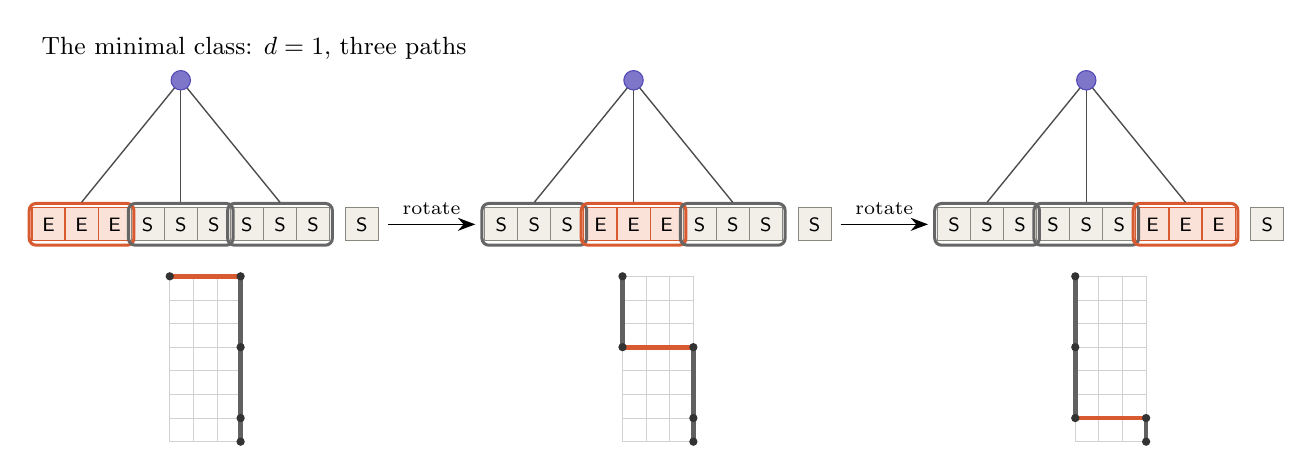
\begin{tikzpicture}
% Generated by gen_figs.py. Claude Fable 5.2 in the Claude app, started by Andrei, 2026-11-14. Not human-reviewed.
\node[ebox] at (0.210,0.210) {\textsf{E}};
\node[ebox] at (0.630,0.210) {\textsf{E}};
\node[ebox] at (1.050,0.210) {\textsf{E}};
\node[sbox] at (1.470,0.210) {\textsf{S}};
\node[sbox] at (1.890,0.210) {\textsf{S}};
\node[sbox] at (2.310,0.210) {\textsf{S}};
\node[sbox] at (2.730,0.210) {\textsf{S}};
\node[sbox] at (3.150,0.210) {\textsf{S}};
\node[sbox] at (3.570,0.210) {\textsf{S}};
\node[sbox] at (4.190,0.210) {\textsf{S}};
\draw[eatom] (-0.035,-0.055) rectangle (1.295,0.475);
\draw[edge] (1.890,2.040) -- (0.630,0.490);
\draw[satom] (1.225,-0.055) rectangle (2.555,0.475);
\draw[edge] (1.890,2.040) -- (1.890,0.490);
\draw[satom] (2.485,-0.055) rectangle (3.815,0.475);
\draw[edge] (1.890,2.040) -- (3.150,0.490);
\node[asymn] at (1.890,2.040) {};
\draw[grid] (1.750,-2.550) -- (1.750,-0.450);
\draw[grid] (2.050,-2.550) -- (2.050,-0.450);
\draw[grid] (2.350,-2.550) -- (2.350,-0.450);
\draw[grid] (2.650,-2.550) -- (2.650,-0.450);
\draw[grid] (1.750,-2.550) -- (2.650,-2.550);
\draw[grid] (1.750,-2.250) -- (2.650,-2.250);
\draw[grid] (1.750,-1.950) -- (2.650,-1.950);
\draw[grid] (1.750,-1.650) -- (2.650,-1.650);
\draw[grid] (1.750,-1.350) -- (2.650,-1.350);
\draw[grid] (1.750,-1.050) -- (2.650,-1.050);
\draw[grid] (1.750,-0.750) -- (2.650,-0.750);
\draw[grid] (1.750,-0.450) -- (2.650,-0.450);
\draw[estep] (1.750,-0.450) -- (2.050,-0.450);
\draw[estep] (2.050,-0.450) -- (2.350,-0.450);
\draw[estep] (2.350,-0.450) -- (2.650,-0.450);
\draw[sstep] (2.650,-0.450) -- (2.650,-0.750);
\draw[sstep] (2.650,-0.750) -- (2.650,-1.050);
\draw[sstep] (2.650,-1.050) -- (2.650,-1.350);
\draw[sstep] (2.650,-1.350) -- (2.650,-1.650);
\draw[sstep] (2.650,-1.650) -- (2.650,-1.950);
\draw[sstep] (2.650,-1.950) -- (2.650,-2.250);
\draw[sstep] (2.650,-2.250) -- (2.650,-2.550);
\fill[black!80] (2.650,-0.450) circle (1.5pt);
\fill[black!80] (2.650,-1.350) circle (1.5pt);
\fill[black!80] (2.650,-2.250) circle (1.5pt);
\fill[black!80] (1.750,-0.450) circle (1.5pt);
\fill[black!80] (2.650,-2.550) circle (1.5pt);
\node[sbox] at (5.960,0.210) {\textsf{S}};
\node[sbox] at (6.380,0.210) {\textsf{S}};
\node[sbox] at (6.800,0.210) {\textsf{S}};
\node[ebox] at (7.220,0.210) {\textsf{E}};
\node[ebox] at (7.640,0.210) {\textsf{E}};
\node[ebox] at (8.060,0.210) {\textsf{E}};
\node[sbox] at (8.480,0.210) {\textsf{S}};
\node[sbox] at (8.900,0.210) {\textsf{S}};
\node[sbox] at (9.320,0.210) {\textsf{S}};
\node[sbox] at (9.940,0.210) {\textsf{S}};
\draw[satom] (5.715,-0.055) rectangle (7.045,0.475);
\draw[edge] (7.640,2.040) -- (6.380,0.490);
\draw[eatom] (6.975,-0.055) rectangle (8.305,0.475);
\draw[edge] (7.640,2.040) -- (7.640,0.490);
\draw[satom] (8.235,-0.055) rectangle (9.565,0.475);
\draw[edge] (7.640,2.040) -- (8.900,0.490);
\node[asymn] at (7.640,2.040) {};
\draw[grid] (7.500,-2.550) -- (7.500,-0.450);
\draw[grid] (7.800,-2.550) -- (7.800,-0.450);
\draw[grid] (8.100,-2.550) -- (8.100,-0.450);
\draw[grid] (8.400,-2.550) -- (8.400,-0.450);
\draw[grid] (7.500,-2.550) -- (8.400,-2.550);
\draw[grid] (7.500,-2.250) -- (8.400,-2.250);
\draw[grid] (7.500,-1.950) -- (8.400,-1.950);
\draw[grid] (7.500,-1.650) -- (8.400,-1.650);
\draw[grid] (7.500,-1.350) -- (8.400,-1.350);
\draw[grid] (7.500,-1.050) -- (8.400,-1.050);
\draw[grid] (7.500,-0.750) -- (8.400,-0.750);
\draw[grid] (7.500,-0.450) -- (8.400,-0.450);
\draw[sstep] (7.500,-0.450) -- (7.500,-0.750);
\draw[sstep] (7.500,-0.750) -- (7.500,-1.050);
\draw[sstep] (7.500,-1.050) -- (7.500,-1.350);
\draw[estep] (7.500,-1.350) -- (7.800,-1.350);
\draw[estep] (7.800,-1.350) -- (8.100,-1.350);
\draw[estep] (8.100,-1.350) -- (8.400,-1.350);
\draw[sstep] (8.400,-1.350) -- (8.400,-1.650);
\draw[sstep] (8.400,-1.650) -- (8.400,-1.950);
\draw[sstep] (8.400,-1.950) -- (8.400,-2.250);
\draw[sstep] (8.400,-2.250) -- (8.400,-2.550);
\fill[black!80] (7.500,-1.350) circle (1.5pt);
\fill[black!80] (8.400,-1.350) circle (1.5pt);
\fill[black!80] (8.400,-2.250) circle (1.5pt);
\fill[black!80] (7.500,-0.450) circle (1.5pt);
\fill[black!80] (8.400,-2.550) circle (1.5pt);
\node[sbox] at (11.710,0.210) {\textsf{S}};
\node[sbox] at (12.130,0.210) {\textsf{S}};
\node[sbox] at (12.550,0.210) {\textsf{S}};
\node[sbox] at (12.970,0.210) {\textsf{S}};
\node[sbox] at (13.390,0.210) {\textsf{S}};
\node[sbox] at (13.810,0.210) {\textsf{S}};
\node[ebox] at (14.230,0.210) {\textsf{E}};
\node[ebox] at (14.650,0.210) {\textsf{E}};
\node[ebox] at (15.070,0.210) {\textsf{E}};
\node[sbox] at (15.690,0.210) {\textsf{S}};
\draw[satom] (11.465,-0.055) rectangle (12.795,0.475);
\draw[edge] (13.390,2.040) -- (12.130,0.490);
\draw[satom] (12.725,-0.055) rectangle (14.055,0.475);
\draw[edge] (13.390,2.040) -- (13.390,0.490);
\draw[eatom] (13.985,-0.055) rectangle (15.315,0.475);
\draw[edge] (13.390,2.040) -- (14.650,0.490);
\node[asymn] at (13.390,2.040) {};
\draw[grid] (13.250,-2.550) -- (13.250,-0.450);
\draw[grid] (13.550,-2.550) -- (13.550,-0.450);
\draw[grid] (13.850,-2.550) -- (13.850,-0.450);
\draw[grid] (14.150,-2.550) -- (14.150,-0.450);
\draw[grid] (13.250,-2.550) -- (14.150,-2.550);
\draw[grid] (13.250,-2.250) -- (14.150,-2.250);
\draw[grid] (13.250,-1.950) -- (14.150,-1.950);
\draw[grid] (13.250,-1.650) -- (14.150,-1.650);
\draw[grid] (13.250,-1.350) -- (14.150,-1.350);
\draw[grid] (13.250,-1.050) -- (14.150,-1.050);
\draw[grid] (13.250,-0.750) -- (14.150,-0.750);
\draw[grid] (13.250,-0.450) -- (14.150,-0.450);
\draw[sstep] (13.250,-0.450) -- (13.250,-0.750);
\draw[sstep] (13.250,-0.750) -- (13.250,-1.050);
\draw[sstep] (13.250,-1.050) -- (13.250,-1.350);
\draw[sstep] (13.250,-1.350) -- (13.250,-1.650);
\draw[sstep] (13.250,-1.650) -- (13.250,-1.950);
\draw[sstep] (13.250,-1.950) -- (13.250,-2.250);
\draw[estep] (13.250,-2.250) -- (13.550,-2.250);
\draw[estep] (13.550,-2.250) -- (13.850,-2.250);
\draw[estep] (13.850,-2.250) -- (14.150,-2.250);
\draw[sstep] (14.150,-2.250) -- (14.150,-2.550);
\fill[black!80] (13.250,-1.350) circle (1.5pt);
\fill[black!80] (13.250,-2.250) circle (1.5pt);
\fill[black!80] (14.150,-2.250) circle (1.5pt);
\fill[black!80] (13.250,-0.450) circle (1.5pt);
\fill[black!80] (14.150,-2.550) circle (1.5pt);
\draw[act] (4.52,0.21) -- node[above,font=\scriptsize]{rotate} (5.63,0.21);
\draw[act] (10.27,0.21) -- node[above,font=\scriptsize]{rotate} (11.38,0.21);
\node[font=\small,anchor=west] at (0,2.45) {The minimal class: $d=1$, three paths};

\end{tikzpicture}

\vspace{1.2em}
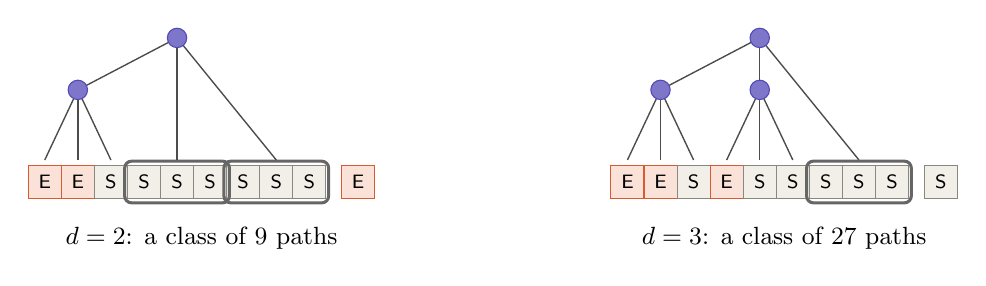
\begin{tikzpicture}
% Generated by gen_figs.py. Claude Fable 5.2 in the Claude app, started by Andrei, 2026-11-14. Not human-reviewed.
\node[ebox] at (1.810,0.210) {\textsf{E}};
\node[ebox] at (2.230,0.210) {\textsf{E}};
\node[sbox] at (2.650,0.210) {\textsf{S}};
\node[sbox] at (3.070,0.210) {\textsf{S}};
\node[sbox] at (3.490,0.210) {\textsf{S}};
\node[sbox] at (3.910,0.210) {\textsf{S}};
\node[sbox] at (4.330,0.210) {\textsf{S}};
\node[sbox] at (4.750,0.210) {\textsf{S}};
\node[sbox] at (5.170,0.210) {\textsf{S}};
\node[ebox] at (5.790,0.210) {\textsf{E}};
\draw[edge] (3.490,2.040) -- (2.230,1.380);
\draw[edge] (2.230,1.380) -- (1.810,0.490);
\draw[edge] (2.230,1.380) -- (2.230,0.490);
\draw[edge] (2.230,1.380) -- (2.650,0.490);
\node[asymn] at (2.230,1.380) {};
\draw[satom] (2.825,-0.055) rectangle (4.155,0.475);
\draw[edge] (3.490,2.040) -- (3.490,0.490);
\draw[satom] (4.085,-0.055) rectangle (5.415,0.475);
\draw[edge] (3.490,2.040) -- (4.750,0.490);
\node[asymn] at (3.490,2.040) {};
\node[font=\small] at (3.80,-0.5) {$d=2$: a class of $9$ paths};
\node[ebox] at (9.210,0.210) {\textsf{E}};
\node[ebox] at (9.630,0.210) {\textsf{E}};
\node[sbox] at (10.050,0.210) {\textsf{S}};
\node[ebox] at (10.470,0.210) {\textsf{E}};
\node[sbox] at (10.890,0.210) {\textsf{S}};
\node[sbox] at (11.310,0.210) {\textsf{S}};
\node[sbox] at (11.730,0.210) {\textsf{S}};
\node[sbox] at (12.150,0.210) {\textsf{S}};
\node[sbox] at (12.570,0.210) {\textsf{S}};
\node[sbox] at (13.190,0.210) {\textsf{S}};
\draw[edge] (10.890,2.040) -- (9.630,1.380);
\draw[edge] (9.630,1.380) -- (9.210,0.490);
\draw[edge] (9.630,1.380) -- (9.630,0.490);
\draw[edge] (9.630,1.380) -- (10.050,0.490);
\node[asymn] at (9.630,1.380) {};
\draw[edge] (10.890,2.040) -- (10.890,1.380);
\draw[edge] (10.890,1.380) -- (10.470,0.490);
\draw[edge] (10.890,1.380) -- (10.890,0.490);
\draw[edge] (10.890,1.380) -- (11.310,0.490);
\node[asymn] at (10.890,1.380) {};
\draw[satom] (11.485,-0.055) rectangle (12.815,0.475);
\draw[edge] (10.890,2.040) -- (12.150,0.490);
\node[asymn] at (10.890,2.040) {};
\node[font=\small] at (11.20,-0.5) {$d=3$: a class of $27$ paths};

\end{tikzpicture}
\caption{Example~\ref{ex:A}. Top: the minimal class, as words and as paths from $(0,7)$ to $(3,0)$. The
$9$-segment is the only mixed segment; its three thirds are atoms. Bottom: paths in two of the larger classes. They are not
minimal because their steps $\E$ are split into three atoms of length $1$, while $n=3=(10)_3$ has digit sum $1$.}
\label{fig:exA}
\end{figure}

\begin{example}[$p=3$, $q=9$, $n=2$]\label{ex:B}
Here $m=17=(122)_3$, $N=19=(201)_3$, $C=\frac1{17}\binom{18}2=9$ and $t=(5-1)/2=2$. The top segments are two
segments of length $9$ and one single step. Adding $n=(2)_3$ and $m=(122)_3$ carries into digits $1$ and $2$.
So a minimal path has one mixed segment of length $9$ and one mixed segment of length $3$ inside it
(Figure~\ref{fig:exB}). The count of Proposition~\ref{prop:count}:

\begin{center}\small
\begin{tabular}{@{}clll@{}}
\toprule
length & slots & to place & ways\\
\midrule
$9$ & the $2$ top segments of length $9$ & one $\Ss$-atom, one mixed & $2!=2$\\
$3$ & the $3$ thirds of the mixed $9$-segment & two $\Ss$-atoms, one mixed & $3!/2!=3$\\
$1$ & the $3$ steps of the mixed $3$-segment, the single step & two $\E$, two $\Ss$ & $4!/(2!\,2!)=6$\\
\bottomrule
\end{tabular}
\end{center}

So there are $2\cdot3\cdot6=36$ minimal paths, in $M=36/3^2=4$ classes. All $\binom{19}2=171$ paths: four classes
of $9$, two of $27$, one of $81$. So $19\cdot C=171=9\cdot4+27\cdot5$, hence $C=9$ and
$C/9=1\equiv4\equiv(-1)^2/(2!\,2!\,1!)\pmod3$.
\end{example}

\begin{figure}[ht]
\centering
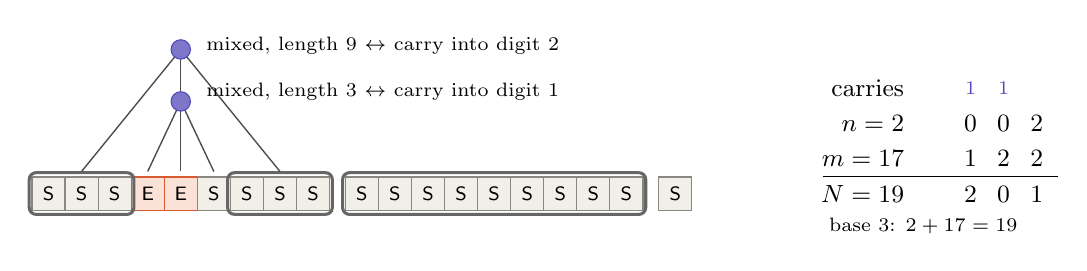
\begin{tikzpicture}
% Generated by gen_figs.py. Claude Fable 5.2 in the Claude app, started by Andrei, 2026-11-14. Not human-reviewed.
\node[sbox] at (0.210,0.210) {\textsf{S}};
\node[sbox] at (0.630,0.210) {\textsf{S}};
\node[sbox] at (1.050,0.210) {\textsf{S}};
\node[ebox] at (1.470,0.210) {\textsf{E}};
\node[ebox] at (1.890,0.210) {\textsf{E}};
\node[sbox] at (2.310,0.210) {\textsf{S}};
\node[sbox] at (2.730,0.210) {\textsf{S}};
\node[sbox] at (3.150,0.210) {\textsf{S}};
\node[sbox] at (3.570,0.210) {\textsf{S}};
\node[sbox] at (4.190,0.210) {\textsf{S}};
\node[sbox] at (4.610,0.210) {\textsf{S}};
\node[sbox] at (5.030,0.210) {\textsf{S}};
\node[sbox] at (5.450,0.210) {\textsf{S}};
\node[sbox] at (5.870,0.210) {\textsf{S}};
\node[sbox] at (6.290,0.210) {\textsf{S}};
\node[sbox] at (6.710,0.210) {\textsf{S}};
\node[sbox] at (7.130,0.210) {\textsf{S}};
\node[sbox] at (7.550,0.210) {\textsf{S}};
\node[sbox] at (8.170,0.210) {\textsf{S}};
\draw[satom] (-0.035,-0.055) rectangle (1.295,0.475);
\draw[edge] (1.890,2.040) -- (0.630,0.490);
\draw[edge] (1.890,2.040) -- (1.890,1.380);
\draw[edge] (1.890,1.380) -- (1.470,0.490);
\draw[edge] (1.890,1.380) -- (1.890,0.490);
\draw[edge] (1.890,1.380) -- (2.310,0.490);
\node[asymn] at (1.890,1.380) {};
\draw[satom] (2.485,-0.055) rectangle (3.815,0.475);
\draw[edge] (1.890,2.040) -- (3.150,0.490);
\node[asymn] at (1.890,2.040) {};
\draw[satom] (3.945,-0.055) rectangle (7.795,0.475);
\node[font=\scriptsize,anchor=west] at (2.09,2.09) {mixed, length $9$ $\leftrightarrow$ carry into digit $2$};
\node[font=\scriptsize,anchor=west] at (2.09,1.50) {mixed, length $3$ $\leftrightarrow$ carry into digit $1$};
\node[font=\small,anchor=east] at (11.20,1.55) {carries};
\node[font=\small] at (11.92,1.55) {\color{purpline}\scriptsize $1$};
\node[font=\small] at (12.34,1.55) {\color{purpline}\scriptsize $1$};
\node[font=\small,anchor=east] at (11.20,1.10) {$n=2$};
\node[font=\small] at (11.92,1.10) {\small $0$};
\node[font=\small] at (12.34,1.10) {\small $0$};
\node[font=\small] at (12.76,1.10) {\small $2$};
\node[font=\small,anchor=east] at (11.20,0.65) {$m=17$};
\node[font=\small] at (11.92,0.65) {\small $1$};
\node[font=\small] at (12.34,0.65) {\small $2$};
\node[font=\small] at (12.76,0.65) {\small $2$};
\node[font=\small,anchor=east] at (11.20,0.20) {$N=19$};
\node[font=\small] at (11.92,0.20) {\small $2$};
\node[font=\small] at (12.34,0.20) {\small $0$};
\node[font=\small] at (12.76,0.20) {\small $1$};
\draw[line width=0.5pt] (10.05,0.43) -- (13.03,0.43);
\node[font=\scriptsize,anchor=west] at (10.00,-0.20) {base $3$: $2+17=19$};

\end{tikzpicture}
\caption{Example~\ref{ex:B}: a minimal path with its two mixed segments, one for each carry of the addition on
the right. Its atoms are two $\E$-atoms of length $1$ and $\Ss$-atoms of lengths $9,3,3,1,1$: the digits of $n=(2)_3$ and
$m=(122)_3$.}
\label{fig:exB}
\end{figure}

\section{Remarks}\label{sec:remarks}

\begin{enumerate}[leftmargin=*,itemsep=4pt]
\item \textbf{What the symmetry acts on.} The moves act on all $N\cdot C$ paths in $\W$. They do not act on the $C$
classes of cyclic shifts, and they do not keep a path under the line of Remark~\ref{rem:dyck}: a move and a cyclic
shift do not commute. The passage from $\binom Nn$ to $C$ uses the free cyclic symmetry (Lemma~\ref{lem:shift}) and
one arithmetic fact, $N\equiv1\pmod p$.

\item \textbf{It is a statement about binomial coefficients.} Sections \ref{sec:moves}--\ref{sec:count} never use
$N=qn+1$. Theorem~\ref{thm:binom} is classical. According to the introduction of \cite{G}, the exponent is Kummer's theorem
(1852), and the congruence was found by Anton (1869), Stickelberger (1890) and Hensel (1902). Theorem~\ref{thm:main} is
its special case $\binom{qn+1}n$. What the argument here adds is a proof by a group action, with the carries
visible as mixed segments. We have not searched the literature properly for this proof. The group-action proof of
Lucas' theorem on the Wikipedia page ``Lucas's theorem'' uses only cyclic rotations of blocks of length $p^i$, not nested ones.
Before any claim of novelty this needs a real search.

\item \textbf{Is it a proof ``from symmetries of trees''?} The group is the rotation group of a forest of
complete $p$-ary trees, a Sylow $p$-subgroup of the symmetric group of the steps. In the tree proof such a group
appears as the symmetry group of a minimal tree (the team's note \texttt{notes/2026-11-14\_connections\_ranked.md},
section 3.2); here it acts from the start. But these are the trees of segments, not the $q$-ary trees that $C$ counts
and on which the group of \cite{K} acts. Whether this answers Problem~137 is for the team to judge.

\item \textbf{Comparison with the tree proof.}\nopagebreak[4]

\nopagebreak[4]\smallskip
{\small
\begin{tabular}{@{}p{0.17\textwidth}p{0.37\textwidth}p{0.37\textwidth}@{}}
\toprule
 & tree proof & path proof\\
\midrule
objects & $k$-blocked $p$-ary trees, $C$ of them & paths, $N\cdot C$ of them\\
symmetry & rotate the children of any node of the tree & rotate the sub-segments of any segment; the segments are fixed\\
class size & $p^{d}$, $d$ = number of asymmetric nodes & $p^{d}$, $d$ = number of asymmetric segments\\
lower bound & $d\ge t$, digit sums of leaf numbers & $d\ge t$, digit sums of step numbers\\
minimal objects & $m_j$ complete subtrees of height $j$ on a skeleton with $t$ asymmetric nodes
 & $m_j$ $\Ss$-atoms and $n_j$ $\E$-atoms of length $p^j$ under $t$ mixed segments\\
minimal classes & $|\mathcal S(m,k)|$, evaluated modulo $p$ by the cherry collapse & an explicit product; Wilson's theorem once for each carry\\
\bottomrule
\end{tabular}}

\smallskip
The last row is the difference. On paths the skeleton is rigid: one mixed segment for each carry, so the minimal
classes can be counted level by level. On trees the shape of the skeleton varies, and the cherry collapse does
the count.

\item \textbf{What was checked by computer.} By brute force over all paths: Lemma~\ref{lem:size} (also by computing the
classes directly from the moves), Proposition~\ref{prop:bound}, Lemma~\ref{lem:mixed}, the exact count \eqref{eq:M}
and Theorem~\ref{thm:binom}, for all $0\le n\le N\le16$ and $p=2,3,5$ ($456$ cases); and Theorem~\ref{thm:main} for $34$
pairs $(q,n)$ with $q\in\{2,3,4,5,7,8,9\}$ and $N\le28$. Also Lemma~\ref{lem:shift} and
Remark~\ref{rem:dyck} for small $(q,n)$. Scripts and their output: \texttt{experiments/path\_segments/} in the folder \texttt{guests/andrei-claude/}.
\end{enumerate}

\begin{thebibliography}{9}\small
\bibitem{K} M.~Konvalinka, Divisibility of generalized Catalan numbers, \emph{Journal of Combinatorial Theory,
Series A} 114 (2007), no.~6, 1089--1100. (Data from the project's \texttt{references/README.md}.)
\bibitem{Kal} L.~Kaloujnine, La structure des $p$-groupes de Sylow des groupes sym\'etriques finis, \emph{Annales
scientifiques de l'\'Ecole Normale Sup\'erieure} (3) 65 (1948), 239--276. (Entry 43 of \texttt{references/README.md}; not opened by us.)
\bibitem{GL} E.~Giannelli and S.~Law, On permutation characters and Sylow $p$-subgroups of $S_n$, arXiv:1712.02642 (2017).
(Entry 44 of \texttt{references/README.md}, where it is noted that $p$ is odd there; not opened by us.)
\bibitem{G} A.~Granville, Arithmetic properties of binomial coefficients I: Binomial coefficients modulo prime
powers, \emph{Canadian Mathematical Society Conference Proceedings} 20 (1997), 253--275. (Found by web search on
14 November 2026; bibliographic data as given on the Wikipedia page ``Lucas's theorem''; only the introduction of the
online version was read. Not in \texttt{references/README.md}; the web version is listed in the team's
\texttt{notes/2026-11-14\_connections\_sources.md}.)
\end{thebibliography}

\end{document}
